\paragraph{QuizziPedia::Front-End::ModelViews::EditorQMLModelView}
\begin{figure} [ht]
	\centering
	%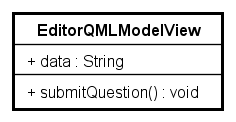
\includegraphics[scale=0.80]{UML/Classi/Front-End/QuizziPedia_Front-end_Views_EditorQMLModelView.png}
	\caption{QuizziPedia::Front-End::ModelViews::EditorQMLModelView}
\end{figure} \FloatBarrier
\begin{itemize}
	\item \textbf{Descrizione}: classe di tipo modelview la cui istanziazione è contenuta all'interno della variabile di ambiente \$scope di \textit{Angular.js\ped{G}}. All'interno di essa sono presenti le variabili e i metodi necessari per il \textit{Two-Way Data-Binding\ped{G}} tra la view \texttt{EditorQMLView} e il controller \texttt{EditorQMLController}; 
	\item \textbf{Utilizzo}: viene utilizzata per effettuare il \textit{Two-Way Data-Binding\ped{G}} tra la view \texttt{EditorQMLView} e il controller \texttt{EditorQMLController} rendendo disponibili variabili e metodi;
	\item \textbf{Relazioni con altre classi}:
	\begin{itemize}
		\item \textit{IN} \texttt{EditorQMLView}: ; 
		\item \textit{IN} \texttt{EditorQMLController}: ;
	\end{itemize}
	\item \textbf{Attributi}:
	\begin{itemize}
		\item
	\end{itemize}
	\item \textbf{Metodi}:
	\begin{itemize}
		\item 
	\end{itemize}
\end{itemize}